\documentclass{standalone}
\usepackage{tikz}
\usetikzlibrary{calc,matrix,decorations.markings,decorations.pathreplacing}
\usetikzlibrary{calc, matrix, positioning}
\usepackage{hsbcommon}

\begin{document}
% \caption{Prisoner’s Dilemma}\label{PD3}
\centering
 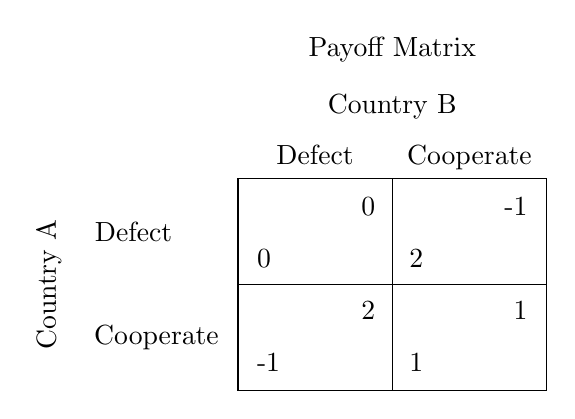
\begin{tikzpicture}
 \matrix[matrix of math nodes,every odd
row/.style={align=right},every even
row/.style={align=left},every node/.style={text width=1.5cm},row
sep=0.2cm,column sep=0.2cm] (m) {
 0&-1\\
 0&2\\
 2&1\\
 -1&1\\
 };
 \draw (m.north east) rectangle (m.south west);
 \draw (m.north) -- (m.south);
 \draw (m.east) -- (m.west);
 \coordinate (a) at ($(m.north west)!0.25!(m.north east)$);
 \coordinate (b) at ($(m.north west)!0.75!(m.north east)$);
 \node[above=5pt of a,anchor=base] {Defect};
 \node[above=5pt of b,anchor=base] {Cooperate};
 \coordinate (c) at ($(m.north west)!0.25!(m.south west)$);
 \coordinate (d) at ($(m.north west)!0.75!(m.south west)$);
 \node[left=20pt of c,align=center,text width=1cm] {Defect};
 \node[left=20pt of d,align=center,text width=1cm] {Cooperate};
 \node[above=18pt of m.north,align=center] (Country b) {Country B};
 \node[left=2.4cm of m.west,rotate=90,align=center,anchor=center]
{Country A};
\node[above=5pt of Country b] {Payoff Matrix};
 \end{tikzpicture}
\end{document}